\chapter{pyNE - General Usage}
\label{Chap:GeneralUsage}
\lettrine[lines=2]{\color{myBrown}\textsf{T}}{}his chapter serves as a brief introduction to the pyNE\footnote{\textbf{py}thon \textbf{N}ano\textbf{E}lectronics} data acquisition software. This quick-start guide will cover the basic structure of the software. For a full list of available instruments, functions and measurement ranges, please refer to Section 2: Instruments, Functions and Ranges.\\
\section{Basic layout of the \textit{control file}}
The \textit{control file} lays out the entire measurement procedure intended by the user. Even though it can be written from scratch quite quickly, it is recommended to save frequently used files in your own private folder.\\
\\
Note: We use the \textit{Spyder} IDE\footnote{Integrated development environment} to edit and execute these files. CTRL+C stops the execution of a running script and thus serves a an emergency stop button.\\
\\
The \textit{control file} has a certain structure in which the desired measurement routine is described. Fig. \ref{Fig:SimpleControl} outlines this for the simple scenario of a single source-drain measurement performed by a Keithley2401. In the header, lines 1-3, we import all the required functions from the main pyNE directory. First of all, the current working directory is changed to the pyNE root folder
\begin{verbatim}
os.chdir('C:\Users\z5168331\Documents\PythonInstrumentControl\Ver1.0')
\end{verbatim}
and afterwards the function '\textit{from Imports import *}' imports all the required files.\\
\\
\begin{figure}[h]
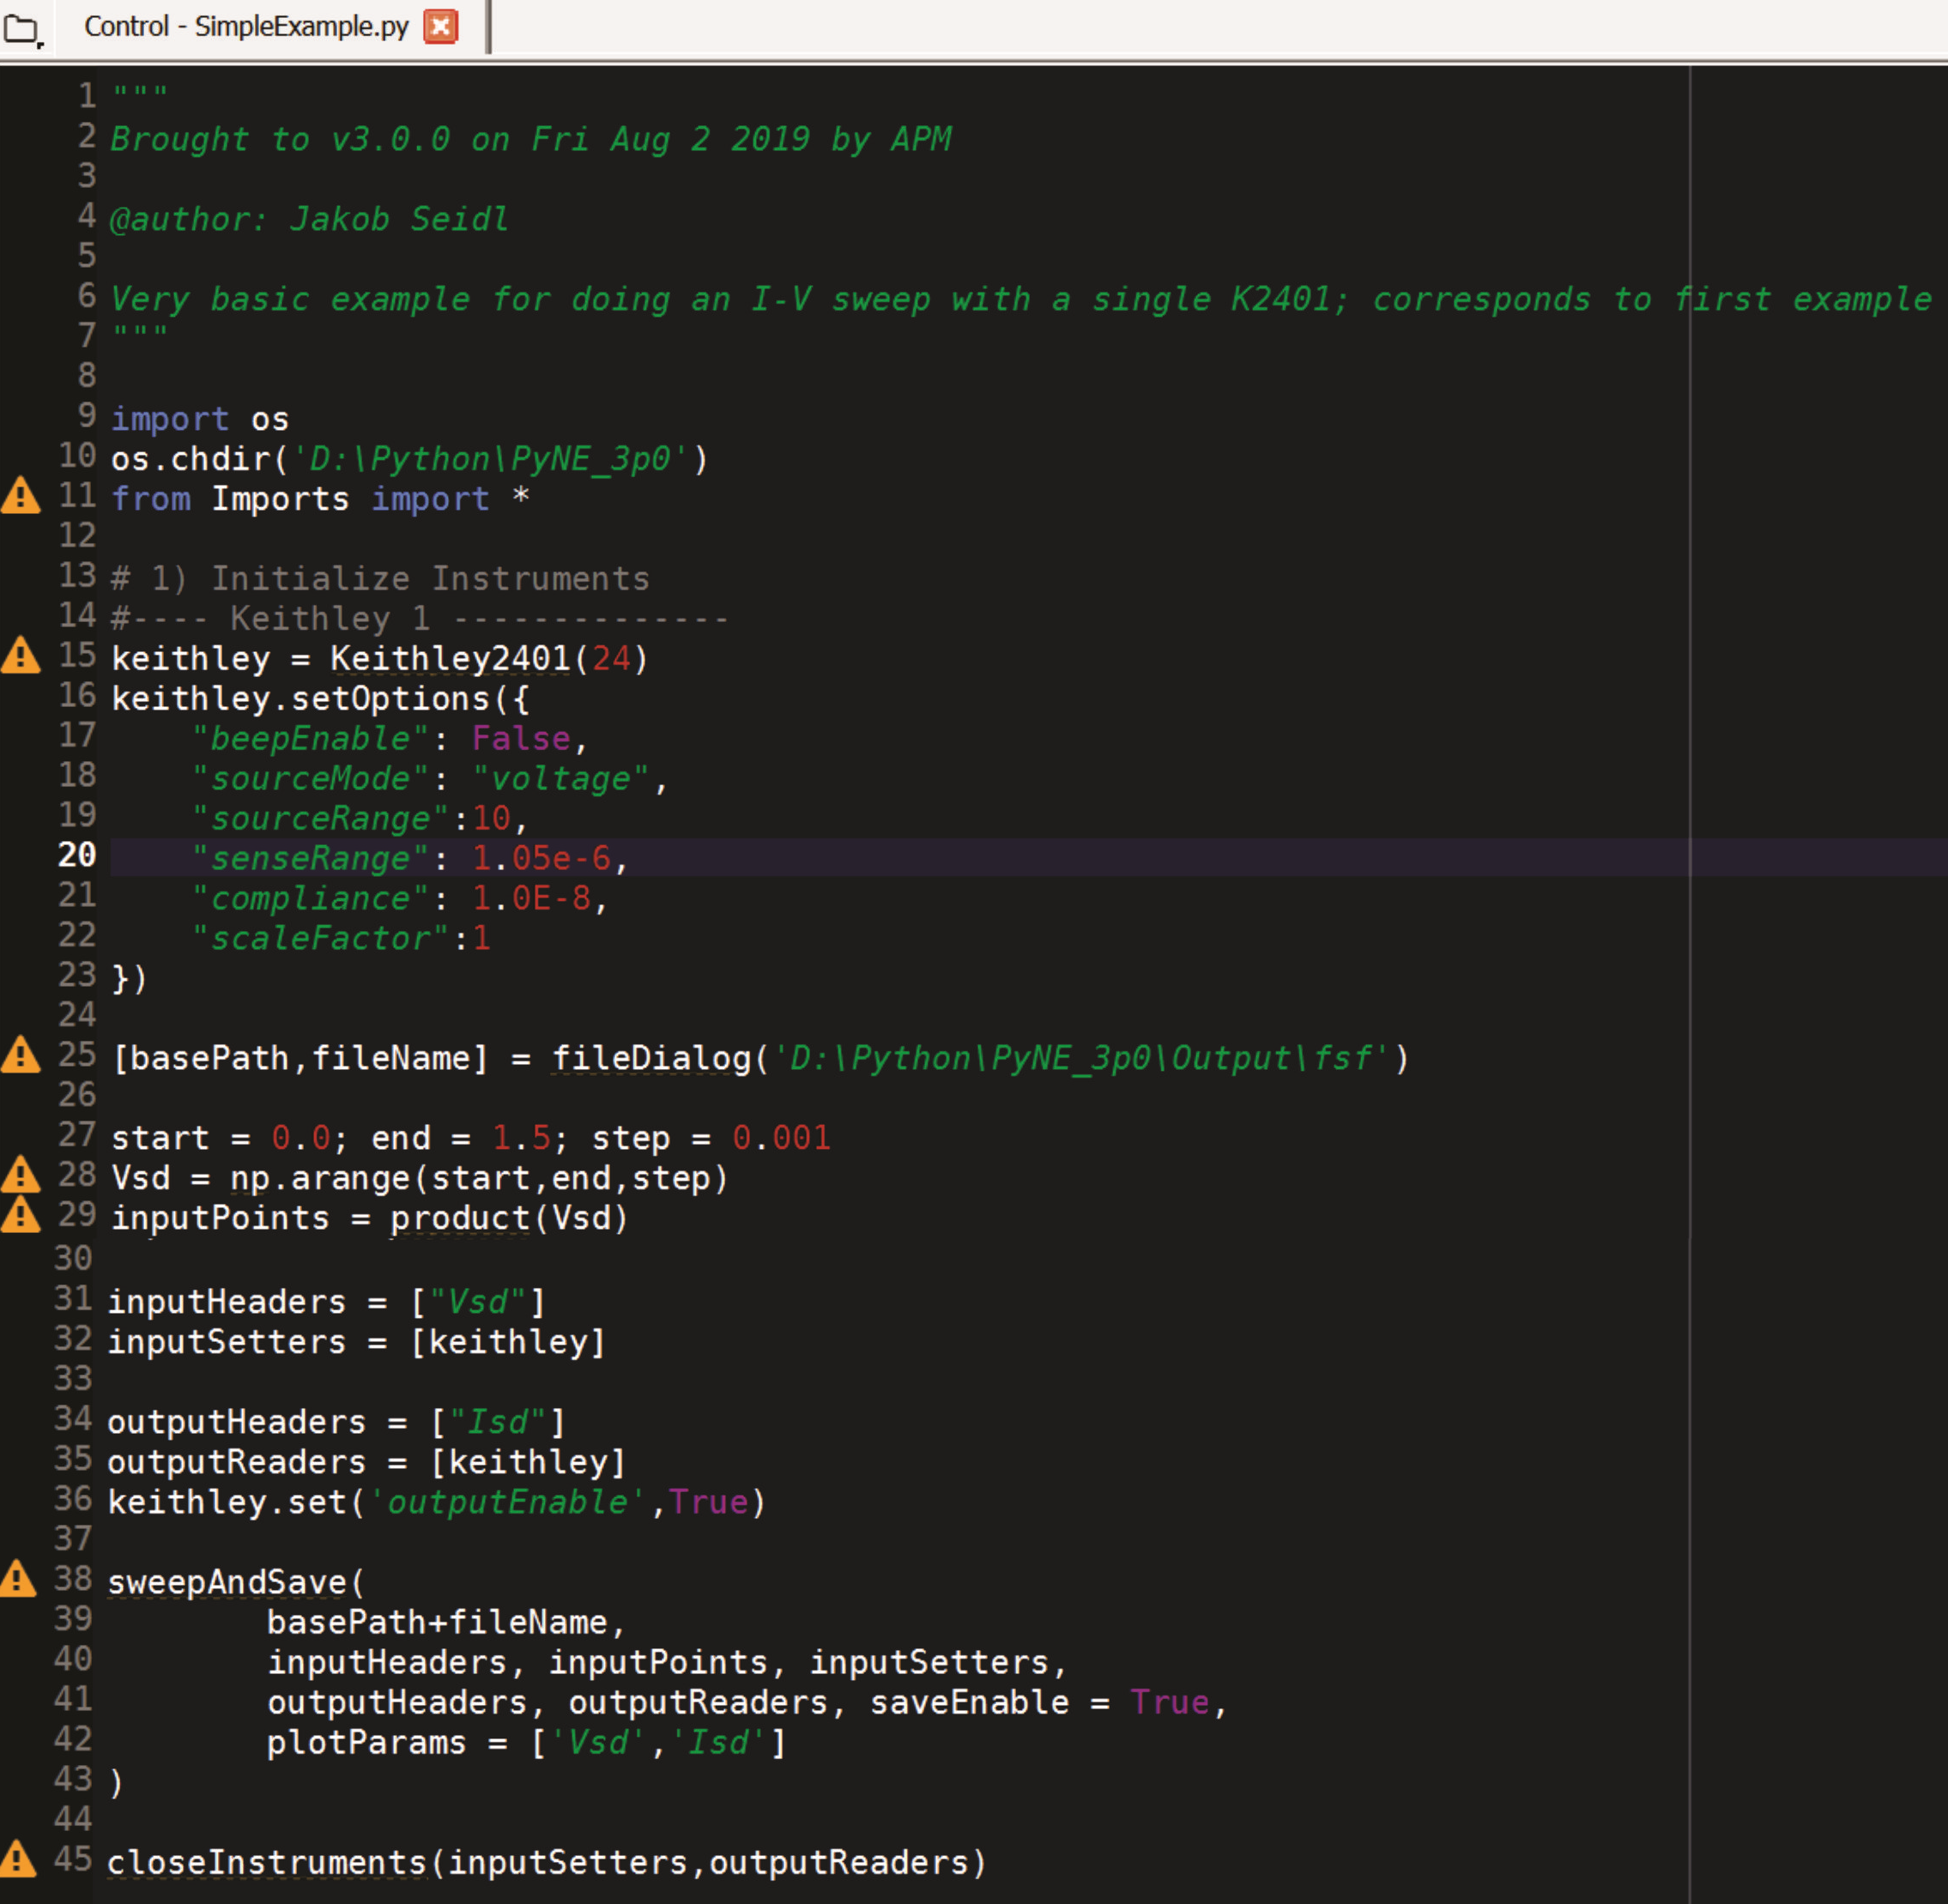
\includegraphics[scale=0.7]{SimpleControl}
\caption{\textbf{Control workflow.} Lines 1-4, import of required functions. Lines 6-14, defines and sets the measurement options for the Keithley2401 object. Line 16 calls a GUI for selecting the results directory and file name. The array of data points we want to sweep over is defined in line 18-19 and subsequently converted into a suitable format in line 20. Lines 22-26 show the setup of input and output headers $\textsf{\&}$ setters (see text). After the output of the SMU is enabled in line 27, the main sweep function is called, lines 29-34. Finally all instrument connections are closed, line 35.}
\label{Fig:SimpleControl}
\end{figure} 
In the next section, the Keithley2401 instrument is defined and connected via
\begin{verbatim}
keithley = Keithley2401(24)
\end{verbatim}
In pyNE, instruments themselves are instances of the corresponding instrument type which are represented by abstract classes. Upon creation, you only have to specify the instrument type (here Keithley2401) and GPIB address (here 24). You can create multiple instruments of the same type (instances) by repeating the above command using a different name and GPIB address, e.g like this: 
\begin{verbatim}
keithley1 = Keithley2401(24)
keithley2 = Keithley2401(11)
\end{verbatim}
Since these instruments are instances of classes, you can use the dot notation (e.g. \texttt{keithley.testFunction(arguments)}) to access the corresponding class functions. These functions represent most basic instrument functionalities you could access from their front panels. The software provides a  couple of higher level functions that execute various low-level functions for you. In this example in lines 7-14, we use the
\begin{verbatim}
instrument.setOptions({
'key1':value1,
'key2':value2
})
\end{verbatim}  function in order to set a couple of options at once. Every instrument has this function but the available options naturally vary from instrument to instrument. The options are formatted in python dictionary format i.e. consist of a \texttt{'key'} with a corresponding \texttt{'value'}. A comprehensive list of all implemented options can be found in Chapter 2. \\
\\
Line 16 opens a short gui-dialog window in which the user specifies the desired base folder and file name for saving his acquired data. These are saved in the variables 'basepath' and 'fileName' which can be overwritten manually by the user at any time, e.g. in order to give certain sweeps completely different file names.\\
\\ 
After all instruments are properly initialized, we can begin to define the parameter space we'd like to sweep through. The \textit{numpy arange}\footnote{\textit{numpy} is commonly imported as 'np' in the python community and we stick to this convention.} is a convenient way of defining an equally spaced array ranging from a start to and end value\footnote{Note that np.arange by default excludes the endpoint!}, cf. lines 18-19. For few discrete points, use a simple python list like 'VSD = [0.2, 0.3, 0.5]' instead. The next line, line 20, converts this newly defined array/list into the format required by the function which performs the actual sweep. It creates an \textit{itertools.product} object. For a single input like here, it will simply be a 1D array. However, when provided two or more inputs, it will create a product array comprised of all the inputs. To give you an example, say you'd like to perform a simple gatesweep measurement for a set of source-drain biases. You'd define the gatesweep range (Vg) just like we've seen before but additionally define ~'VSD = [0.2, 0.3, 0.5]'. \texttt{InputPoints = product(VSD,Vg)} would then span your entire (2D) parameter space, i.e. do one full Vg sweep for Vsd=0.2V, one for 0.3V and one for 0.5V; the order in which the inputs are placed matters here. The keyword \texttt{inputPoints} has been established as the keyword for the final array. This is, of course, pure convention and may be changed at any point.\\
\\
After initializing the instrument(s) and setting the sweep parameter space, we can now declare which of these instruments are going to actually do the sweep, i.e. output values (referred to as \textit{setters}) or which instruments measure input voltages/currents (\textit{readers}). At the same time we define how we want to call the parameters that are sourced or acquired. This is done via the \textit{headers} which exist for the swept variables (\textit{inputHeaders}) and measured data (\textit{outputHeaders}). If you have multiple instruments you define these via a simple list like inputSetters = [keithley,yokogawa]; the same holds for the corresponding headers. Make sure that the order in which the headers and setters are defined matches. The first setter will always be identified with the first header and so forth; avoid errors here since they will at least create a lot of confusion in your data files. Some instruments return two values when measuring (e.g. lock-in amplifiers). Use additional brackets [...] to denote this pair of variables, e.g. like this:
\begin{verbatim}
outputHeaders = [[Ix,Iy],GateLeakage]
outputReaders = [LockIn1,Keithley_Vg]
\end{verbatim}
Finally, after declaring input and output instruments and variables, we then pass all these variables to the main function which performs the sweep for us:
\begin{verbatim}
sweepAndSave(
    basePath+fileName,
    inputHeaders, inputPoints, inputSetters,
    outputHeaders, outputReaders,saveEnable = True,breakCondition = breakCond,
    plotParams = ['Vsd','Isd']
)
\end{verbatim} 
Let's quickly go through the input variables: 
\begin{enumerate}
\item The full file path. Note that strings can just be added in python and thus basePath+fileName is just a string.
\item inputHeaders, inputPoints and inputSetters. These variables were defined above and specify instruments and values that are actively sourced.
\item outputHeaders, outputReaders. As defined above, these specify all instruments and quantities that are read/measured.
\item saveEnable is a boolean (True or False) that decided whether the obtained data will be saved (as .tsv and .mat file) or not.
\item breakCondition = breakCondition is still in the making and thus not yet implemented. You can just leave it out for now.
\item plotParams denotes the variables among inputHeaders and putputHeaders you want to get plotted while measuring. As of yet, you can specify two pairs of variables, i.e. obtain two live plots. Note however, that the first variable is always plotted on the x-axis and must come from the \texttt{inputHeaders}  while the second (y-axis) should be chosen from the range of \texttt{outputHeaders}.
\end{enumerate}
The sweepAndSave() function will do the rest, i.e. slowly sweep all the setters to their initial sweep point (to avoid abrupt changes) and then carry out the sweep. Finally,
\begin{verbatim}
closeInstruments(inputSetters,outputReaders)
\end{verbatim}
will close the connection to all your instruments, as long as they are included in either inputSetter or outoutReaders. You can also manually close any instrument by typing:
\begin{verbatim}
instrument.close()
\end{verbatim}
\section{A more complex example - combining measurements}
After we've understood how to construct a simple measurement in our control file, it is time to move on to a more sophisticated example. Here we will combine \textit{$I_d$ vs. $V_{sd}$} measurement with a set of subsequent \textit{$I_d$ vs. $V_g$} gatesweeps. 
\scriptsize
\begin{verbatim}
import os
os.chdir('C:\Users\Probestation\Desktop\pyNE\Ver1.0')
from Imports import *
#----Keithley Vsd --------------
Ksd = Keithley2401(24)
Ksd.setOptions({
    "beepEnable": False,
    "sourceMode": "voltage",
    "sourceRange":1,
    "senseRange": 1.05e-5,
    "compliance": 1.0E-5,
    "scaleFactor":1
})
#---Keithley Vg -----------
KVg = Keithley2401(11)
KVg.setOptions({
    "beepEnable": False,
    "sourceMode": "voltage",
    "sourceRange":1,
    "senseRange": 1.05e-6,
    "compliance": 1.0E-7,
    "scaleFactor":1
})
#Electrometer
eMeter = Keithley6517A(20)
eMeter.setOptions({
    "autoRange":True,
    'senseRange':2E-6,
   'senseMode':'current',
})
[basePath,fileName] = fileDialog()
#Vsd array
start = -0.05; end = 0.5; step = 0.001  #Create a up and downsweep array
VsdUp = np.arange(start, end, step) #Only the upsweep
VsdDown = np.arange(end, start-step, -step)
VsdUpDown = np.concatenate((VsdUp, VsdDown))  #np.concatenate() fuses two arrays to one

#Gatesweep array, Vg
start = 0.0; end = 1.4; step = 0.005  #Create a up and downsweep array
Vg = np.concatenate((  #np.concatenate() fuses two arrays to one
    np.arange(start, end, step),
    np.arange(end, start-step, -step)
))
#--------------Headers and setters for IV curves
inputHeaders = ["Vsd"]
inputSetters = [Ksd]

outputHeaders = ["Id","Idrough"]
outputReaders = [eMeter,Ksd]

Ksd.set('outputEnable',True)
for i in range(3):  # 3 Vsd sweeps from -0.05 -> 0.05 V
    inputPoints = product(VsdUpDown)
    sweepAndSave(
        basePath+fileName,
        inputHeaders, inputPoints, inputSetters,
        outputHeaders, outputReaders,saveEnable = True,plotParams = ['Vsd','Id']
    )
Ksd.goTo(0.05,delay=0.001) # since we stop the sweep at -0.05 V we go to 0.05 V manually

#--------------Headers and setters for Vg curves
inputHeaders = ["Vg"]
inputSetters = [KVg]

outputHeaders = ["Id","Ileak","Idrough"]
outputReaders = [eMeter,KVg,Ksd]

for i in range(5): # do 5 full gatesweeps from 0 to 1.4 V
    inputPoints = product(Vg)
    sweepAndSave(
        basePath+fileName,
        inputHeaders, inputPoints, inputSetters,
        outputHeaders, outputReaders,saveEnable = True,plotParams = ['Vg','Id','Vg','Ileak']
    )
Ksd.goTo(0.00,delay=0.001)
closeInstruments(inputSetters,outputReaders)
\end{verbatim}
\normalsize
Here, we import three instruments, two Keithley2401 source-measure units (SMUs) and one Keithley6517A electrometer measuring unit. After connecting all required instruments and setting them up, we define both arrays for the gate voltage $V_{\mathrm{g}}$ as well as the source-drain bias $V_{\mathrm{sd}}$. The \texttt{np.concatenate()} function helps by fusing two arrays into one. This allows for up and downsweeps with using just one array or using a higher point-spacing in certain parts of the sweep than in others\footnote{E.g. you could have a coarse spacing in the uninteresting regions of a gatesweep measurement and a very fine one in the transition region.}.\\
\\
The headers and setters must be defined separately for each measurement since it is other instruments sourcing the voltages/currents for each of these measurements. Besides, you might also want to measure different variables and call them differently.\\
\\
Two las things I'd like to draw your attention to:\\
Any setter instrument can be swept to any (sensible) value with
\begin{verbatim}
instrument.goTo(targetValue,stepsize,delay)
\end{verbatim} 
which we use before performing the gate sweep in order to sweep the source-drain bias back from -0.05$\;$V to 0.05$\;$V. Note also the use of \textit{for loops} in this script. These provide a very simple handle on how often we'd like to perform a sweep. This is just a very simple example, in principle one could combine \textit{for} an \textit{while} loops with different conditions based on measurement outcomes, thus creating very sophisticated measurement routines.\\
\\



